\documentclass[12pt]{report}
\usepackage[utf8]{inputenc}
\usepackage[russian]{babel}
%\usepackage[14pt]{extsizes}
\usepackage{listings}
\usepackage{graphicx}
\usepackage{amsmath,amsfonts,amssymb,amsthm,mathtools} 
\usepackage{pgfplots}
\usepackage{filecontents}
\usepackage{indentfirst}
\usepackage{eucal}
\usepackage{enumitem}
\frenchspacing

\usepackage{indentfirst} % Красная строка


\usetikzlibrary{datavisualization}
\usetikzlibrary{datavisualization.formats.functions}

\usepackage{amsmath}




% Для листинга кода:
\lstset{ %
language=python,                 % выбор языка для подсветки
basicstyle=\small\sffamily, % размер и начертание шрифта для подсветки кода
numbers=left,               % где поставить нумерацию строк (слева\справа)
numberstyle=\tiny,           % размер шрифта для номеров строк
stepnumber=1,                   % размер шага между двумя номерами строк
numbersep=5pt,                % как далеко отстоят номера строк от подсвечиваемого кода
showspaces=false,            % показывать или нет пробелы специальными отступами
showstringspaces=false,      % показывать или нет пробелы в строках
showtabs=false,             % показывать или нет табуляцию в строках
frame=single,              % рисовать рамку вокруг кода
tabsize=2,                 % размер табуляции по умолчанию равен 2 пробелам
captionpos=t,              % позиция заголовка вверху [t] или внизу [b] 
breaklines=true,           % автоматически переносить строки (да\нет)
breakatwhitespace=false, % переносить строки только если есть пробел
escapeinside={\#*}{*)}   % если нужно добавить комментарии в коде
}

\usepackage[left=2cm,right=2cm, top=2cm,bottom=2cm,bindingoffset=0cm]{geometry}
% Для измененных титулов глав:
\usepackage{titlesec, blindtext, color} % подключаем нужные пакеты
\definecolor{gray75}{gray}{0.75} % определяем цвет
\newcommand{\hsp}{\hspace{20pt}} % длина линии в 20pt
% titleformat определяет стиль
\titleformat{\chapter}[hang]{\Huge\bfseries}{\thechapter\hsp\textcolor{gray75}{|}\hsp}{0pt}{\Huge\bfseries}


% plot
\usepackage{pgfplots}
\usepackage{filecontents}
\usetikzlibrary{datavisualization}
\usetikzlibrary{datavisualization.formats.functions}

\begin{document}
\thispagestyle{empty}
\begin{titlepage}
	\noindent \begin{minipage}{0.15\textwidth}
	
\includegraphics[width=\linewidth]{b_logo}
	\end{minipage}
	\noindent\begin{minipage}{0.9\textwidth}\centering
		\textbf{Министерство науки и высшего образования Российской Федерации}\\
		\textbf{Федеральное государственное бюджетное образовательное учреждение высшего образования}\\
		\textbf{~~~«Московский государственный технический университет имени Н.Э.~Баумана}\\
		\textbf{(национальный исследовательский университет)»}\\
		\textbf{(МГТУ им. Н.Э.~Баумана)}
	\end{minipage}
	
	\noindent\rule{18cm}{3pt}
	\newline\newline
	\noindent ФАКУЛЬТЕТ $\underline{\text{«Информатика и системы управления»}}$ \newline\newline
	\noindent КАФЕДРА $\underline{\text{«Программное обеспечение ЭВМ и информационные технологии»}}$\newline\newline\newline\newline\newline
	
	
	\begin{center}
		\noindent\begin{minipage}{1.3\textwidth}\centering
			\Large\textbf{  Отчет по лабораторной работе №5}\newline
			\textbf{по дисциплине "Анализ алгоритмов"}\newline\newline
		\end{minipage}
	\end{center}
	
	\noindent\textbf{Тема} $\underline{\text{Конвейерная обработка данных}}$\newline\newline
	\noindent\textbf{Студент} $\underline{\text{Андрич К. }}$\newline\newline
	\noindent\textbf{Группа} $\underline{\text{ИУ7И-56Б}}$\newline\newline
	\noindent\textbf{Оценка (баллы)} $\underline{\text{~~~~~~~~~~~~~~~~~~~~~~~~~~~}}$\newline\newline
	\noindent\textbf{Преподаватели} $\underline{\text{Волкова Л.Л.}}$\newline\newline\newline
	
	\begin{center}
		\vfill
		Москва~---~\the\year
		~г.
	\end{center}
\end{titlepage}


\tableofcontents

\newpage
\chapter*{Введение}
\addcontentsline{toc}{chapter}{Введение}
Имеется большое количество важнейших задач, решение которых
требует использования огромных вычислительных мощностей, зачастую
недоступных для современных вычислительных систем.
Постоянно появляются новые задачи подобного рода и возрастают
требования к точности и к скорости решения прежних задач; поэтому вопросы разработки и использования сверхмощных компьютеров (называемых суперкомпьютерами) актуальны сейчас и в будущем. Но пока эти
трудности пока что не удается преодолеть. Из-за этого приходится и эти по
пути создания параллельных вычислительных систем, т.е. систем, в которых предусмотрена одновременная реализация ряда вычислительных процессов, связанных с решением одной задачи. На современном этапе развития вычислительной техники такой способ, по-видимому, является одним
из основных способов ускорения вычислений.
\newline

Цель данной лабораторной работы: получить навык организации асинхронной передачи данных между потоками на примере конвейерной обработки информации.
\newline

Для достижения поставленной цели требуется выполнить следующие задачи.
\begin{enumerate}
	\item Выбрать и описать методы обработки данных, которые будут сопоставлены методам конвейера.
	
	\item Описать архитектуру программы, а именно какие функции имеет главный поток, принципы и алгоритмы обмена данными между потоками.
	
	\item Реализовать конвейерную систему, а также сформировать лог событий с указанием времени их происхождения, описать реализацию.
	
	\item Провести тестирование системы.
	
	\item Интерпретировать сформированный лог.
	
\end{enumerate}

Одной из важнейших идей при создании многопроцессорных систем и при эффективной реализации алгоритмов на этих системах является идея конвейерных вычислений.

\chapter{Аналитическая часть}

В данном разделе будут описаны задачи и идея конвейеризации.

\section{Описание задачи}

Конвейеризация – это техника, в результате которой  задача или  команда разбивается  на некоторое число подзадач, которые  выполняются последовательно. Каждая  подкоманда   выполняется на своем логическом  устройстве.    Все     логические    устройства   (ступени)  соединяются последовательно таким образом, что выход  i-ой   ступени   связан   с   входом   (i+1)-ой   ступени,  все ступени  работают  одновременно.  Множество  ступеней называется    конвейером.    Выигрыш     во    времени достигается при  выполнении  нескольких задач  за  счет параллельной   работы   ступеней,  вовлекая  на  каждом такте новую задачу или команду.

В конвейере различают r последовательных этапов, так что когда $i$-я операция проходит $s$-й этап, то $(i+k)$-я операция проходит $(s-k)$-й этап. На рисунке \ref{fig:conv} изображена работа конвейера.

\begin{figure}[h]
	\center{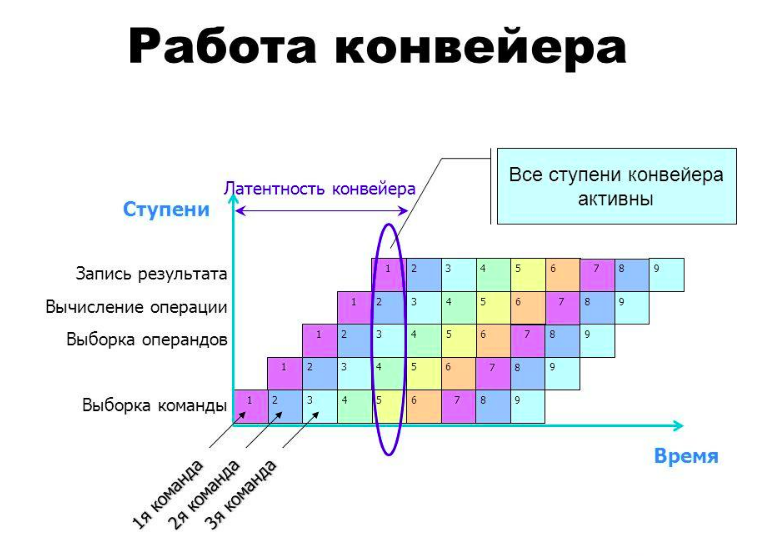
\includegraphics[scale=0.6]{conv.png}}
	\caption{Работа конвейера.}
	\label{fig:conv}
\end{figure}

В данной лабораторной работе реализована некая функцию кодирования строки, которая состоит из трех последовательных действий: применения первой функции шифра Цезаря, применения функции которая меняет регистр буквы и применения функции которая меняет элемент местами с элементом, стоящим на n / 2 от него, где n - размер строки. Если необходимо закодировать какой-то массив строк, то можно использовать конвейерную обработку данных. Таким образом задача будет решена эффективнее, чем при последовательном применении алгоритмов к массиву значений.  

Конвейер будет состоять из четырех уровней. Обработанные данные передаются последовательно с одного уровня (одной ленты) конвейера на следующий (следующую ленту). Далее на каждом уровне осуществляется обработка данных, занимающая определенное время. Для каждой ленты создается своя очередь задач, в которой хранятся все необработанные строки. На последнем уровне конвейера обработанные объекты попадают в пул обработанных задач.

Уровни конвейера: 
\begin{itemize}
	\item 0 уровень — генерация входных данных в первую очередь;
	
	\item 1 уровень(лента) — применение шифра Цезаря к строкам из первой очереди, запись результата во 2 очередь; 
	
	\item 2 уровень(лента) — применение функции, меняющей регистры символов к строкам 2 очереди, запись результата в 3 очередь;
	
	\item 3 уровень(лента) — применение функции, меняющей местами символы в строке по определённом выше закону  к строкам 3 очереди, запись результата в пул обработанных задач.
\end{itemize}

Поскольку запись в очередь и извлечение из очереди это не атомарные операции, необходимо создать их таковыми путем использования мьютексов (по одному на одну очередь) и критических секций, чтобы избежать ошибок в ситуации гонок. 

\section{Вывод}
	В данном разделе были заданы задачи и описана идея конвейеризации.
	
\clearpage

\chapter{Конструкторская часть}

\section{Описание архитектуры ПО}
В конвейере 3 основные ленты, содержание их работы описано выше, в аналитической части отчета. Каждой ленте выделен свой поток, в котором она выполняется. В главном потоке (функция main) создаются три рабочих потока: по одному на каждую ленту. 
Для каждой ленты есть своя очередь, однако с ней могут работать все потоки, поэтому при доступе к элементам очереди необходимо блокировать доступ для других потоков. Для реализации доступа из разных потоков используются мьютексы, по одному для каждой очереди и для результирующего массива создан. 
Также в главном потоке генерируется массив входных данных и заполняется первая очередь (уровень 0).
В рабочих процессах считывается по одному элементу из соответствующей очереди, выполняется вызов обрабатывающих функций, замеры времени и задержка по времени. После обработки текущей задачи, рабочий процесс записывает результат в следующую очередь или в результирующий массив. Также выполняется запись в лог-файл. 

На рисунке \ref{fig:conv_1} изображена схема работы конвейерной обработки.


\begin{figure}[h]
	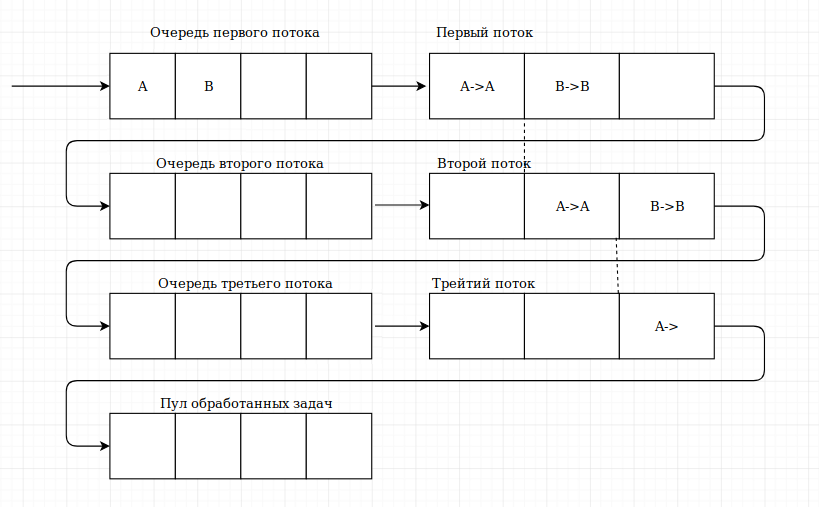
\includegraphics[scale=0.5]{conv1.png}
	\caption{Схема работы конвейерной обработки.}
	\label{fig:conv_1}
\end{figure}

\section{Cхемы алгоритмов работы конвейерной обработки}
На рисунках \ref{fig:main} и \ref{fig:proc} показаны схем главного и рабочего процессов.

\begin{figure}[h]
	\centering
	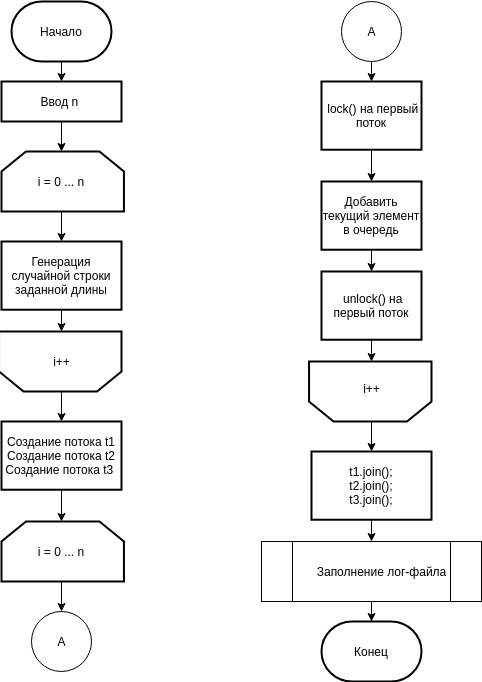
\includegraphics[width=0.6\linewidth]{main_fl.png}
	\caption{Схема работы главного процесса}
	\label{fig:main}
\end{figure}

\newpage

\begin{figure}[h]
	\centering
	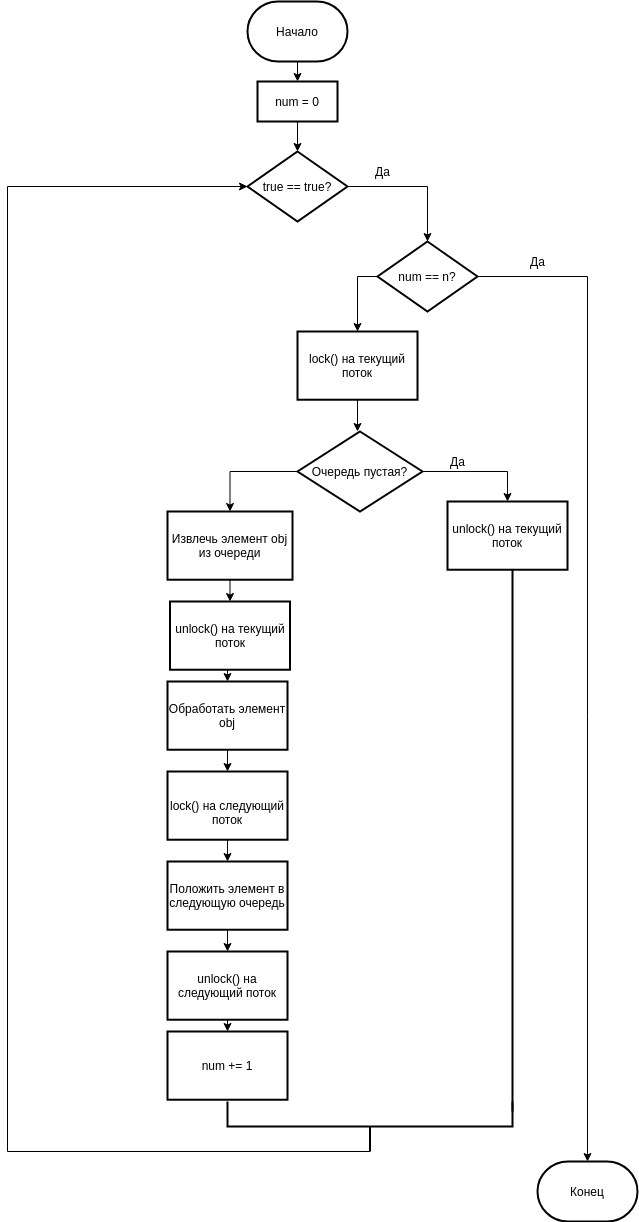
\includegraphics[scale=0.4]{proc.png}
	\caption{Схема работы рабочего процесса}
	\label{fig:proc}
\end{figure}

\section{Вывод}
	В данном разделе показаны схемы рабочего и главного процессов.

\chapter{Технологическая часть}

В этом разделе будет обоснован выбор языка програмирования и приведены листинги кода реализованных алгоритмов.

\section{Выбор ЯП}
В качестве языка программирования был выбран С++ так как этот язык удобен для работы с потоками.
Для замера времени выполнения использовалась функция $clock()$ из библиотеки ctime. Эта функция возвращает количество временных тактов, прошедших с начала запуска программы. 

\section{Реализация алгоритмов}

В листингах \ref{lst:conv1}, \ref{lst:conv2}, \ref{lst:conv3} представлен код рабочих потоков, в листинге \ref{lst:main} представлен код главного потока.
\newpage

\begin{lstlisting}[label={lst:conv1},caption=Реализация первого уровня конвейера.]
	void first_conv() {
		int num = 0;
		while (true) {
			if (num == n)
				break;
			m1.lock();
			if (queue1.empty()) {
				m1.unlock();
				continue;
			}
			string cur_str = queue1.front().str;
			int cur_task_num = queue1.front().task_num;
			timer.add_time(1, clock() - queue1.front().time, queue1.front().task_num);
			queue1.pop();
			
			clock_t cur_time = clock();
			m1.unlock();
			string new_str = caesar(cur_str);
			m2.lock();
			timer.add_time(0, clock() - cur_time, cur_task_num);
			
			queue2.push(Object(new_str, cur_task_num,clock()));
			m2.unlock();
			num++;
		}
	}
\end{lstlisting}
\newpage

\begin{lstlisting}[label={lst:conv2},caption=Реализация второго уровня конвейера.]
	void second_conv() {
		int num = 0;
		while (true) {
			if (num == n)
				break;
			m2.lock(); // wait in queue
			if (queue2.empty()) {
				m2.unlock();
				continue;
			}
			string cur_str = queue2.front().str;
			int cur_task_num = queue2.front().task_num;
			timer.add_time(1, clock() - queue2.front().time, queue2.front().task_num);
			queue2.pop();
			
			clock_t cur_time = clock();
			m2.unlock();
			string new_str = upper_lower(cur_str);
			m3.lock();
			timer.add_time(0, clock() - cur_time, cur_task_num);
			
			queue3.push(Object(new_str, cur_task_num, clock()));
			m3.unlock();
			num++;
		}
	}
	
\end{lstlisting}
\newpage

\begin{lstlisting}[label={lst:conv3},caption=Реализация третьего уровня конвейера.]
	void third_conv() {
		int num = 0;
		while (true) {
			if (num == n)
				break;
			m3.lock(); // wait in queue
			if (queue3.empty()) {
				m3.unlock();
				continue;
			}
			string cur_str = queue3.front().str;
			int cur_task_num = queue3.front().task_num;
			timer.add_time(1, clock() - queue3.front().time, queue3.front().task_num);
			queue3.pop();
			
			clock_t cur_time = clock();
			m3.unlock();
			string new_str = reverse(cur_str);
			resm.lock();
			timer.add_time(0, clock() - cur_time, cur_task_num);
			
			res.push_back(new_str);
			resm.unlock();
			num++;
		}
	}
\end{lstlisting}
\newpage

\begin{lstlisting}[label={lst:main},caption=Основная функция программы.]
	int main() {
		srand(time(nullptr));
		cout << "Enter the number of lines: ";
		cin >> n;
		if (n <= 0) {
			cout << "Incorrect number of lines";
			return -1;
		}
		
		objvec.resize(n);
		timer.set_size();
		
		for (int i = 0; i < n; i++) {
			string s = generate();
			objvec[i] = (s);
		}
		
		start_t = clock();
		
		thread t1(first_conv);
		thread t2(second_conv);
		thread t3(third_conv);
		
		for (int i = 0; i < n; i++) {
			m1.lock();
			queue1.push(Object(objvec[i], i, clock()));
			m1.unlock();
		}
		
		t1.join();
		t2.join();
		t3.join();
		
		create_log(clock() - start_t);
		return 0;
	}
\end{lstlisting}

\section{Тестирование программы}
На вход подаем 6 строк длиной 50000. Программа выдала файл с логом.

\section{Вывод}
В этом разделе обоснован выбор языка програмирования и приведены листинги кода реализованных алгоритмов. Программа прошла тестирование и работает правильно.

\chapter{Исследовательская часть}

В данном разделе будут приведены демонстрация работы программы и исследование процессорного времени реализаций алгоритмов.

\section{Пример работы}

Демонстрация работы программы приведена на рисунке \ref{fig:prog_show}. На вход подаётся количество строк для обработки.

\begin{figure}[h]
	\begin{center}
	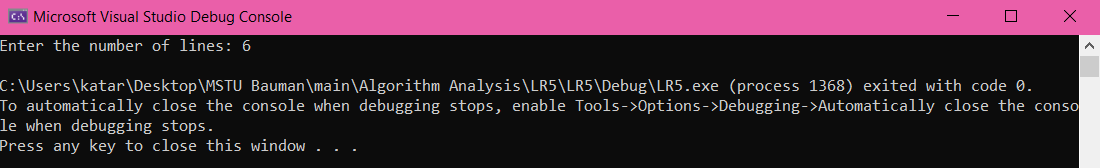
\includegraphics[scale=0.8]{example.png}
	 \caption{Демонстрация работы программы}
	 \label{fig:prog_show}
	\end{center}
\end{figure}

В результате работы программы заполняется лог-файл. Содержимое лог-файла приведено на рисункe \ref{fig:log1}. Время замерено с тактах процессора.

\begin{figure}[h]
	\begin{center}
		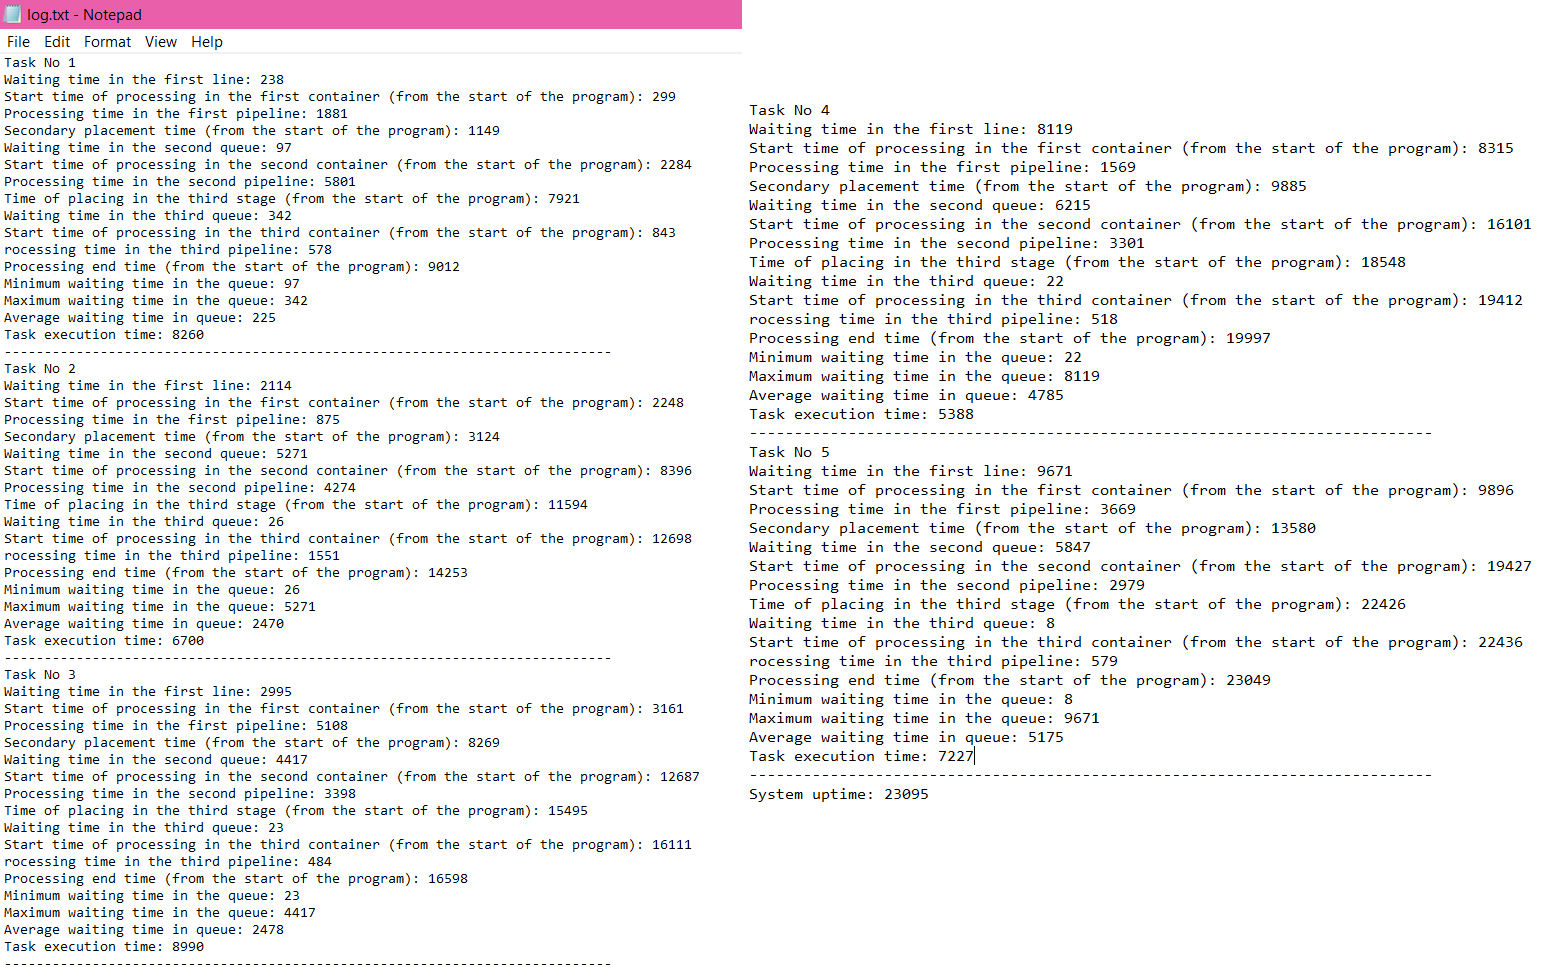
\includegraphics[scale=0.5]{logs.png}
		\caption{Содержимое лог-файла}
		\label{fig:log1}
	\end{center}
\end{figure}
\newpage

По лог-файлу можно проследить выполнение каждого этапа  задач. Также можно проследить, что обработка выполняются параллельно. Например, второй коневейер не ждёт полного завершения работы первого конвейера прежде, чем начать работу, а начинает выполнение как только в очередь поступает первый элемент.

Если бы использовалась линейная реализация, то проделанная работа заняла бы 36656 тактов процессора, что в 1,5 раза больше, чем время, потраченное при конвейерной реализации.
\newpage

\section{Вывод}
Конвейерная обработка данных - полезный инструмент, который уменьшает время выполнения программы за счёт параллельной обработки данных. Самым эффективным временем считается время, когда все линии конвейера работают параллельно, обрабатывая свои задачи. Этот метод даёт выйгрыш по времени в том случае, когда выполняемые задачи намного больше по времени, чем время, затрачиваемое на реализацию конвейера (работу с потоками, перекладывание из очереди в очередь и тд).



\chapter*{Заключение}
\addcontentsline{toc}{chapter}{Заключение}

В ходе лабораторной работы была достигнута цель. Был получен навык организации асинхронной передачи данных между потоками на примере конвейерной обработки информации.

Для достижения поставленной цели были выполнены следующие задачи.
\begin{enumerate}
	\item Выбраны и описаны методы обработки данных, которые будут сопоставлены методам конвейера.
	
	\item Описана архитектура программы, а именно какие функции имеет главный поток, принципы и алгоритмы обмена данными между потоками.
	
	\item Реализована конвейерная система, а также сформирован лог событий с указанием времени их происхождения, описана реализация.
	
	\item Проведено тестирование системы.
	
	\item Интерпретирован сформированный лог.
	
\end{enumerate}

Эксперементальным путём выявлено, что при большой нагрузке конвейер работает примерно в 1,5 раза быстрее чем линейная реализация, что является показателем эффективности работы конвейера по времени.

\addcontentsline{toc}{chapter}{Список литератури}

\bibliographystyle{utf8gost705u}  % стилевой файл для оформления по ГОСТу

\bibliography{51-biblio}          % имя библиографической базы (bib-файла)

\begin{thebibliography}{9}
		
		\bibitem{Voevodin} Воеводин В.В. Математические модели и методы в параллельных процессах. М., 1986. 296с.
		
		\bibitem{Corneev} Корнеев В.В. Параллельные вычислительные системы. М., 1999. 320 с.
		
		\bibitem{conv}  Конвейерные вычисления [Электронный ресурс]. Режим доступа: http://www.myshared.ru/slide/674082 Дата обращения: 31.10.2021
		
		\bibitem{ctime} Функция clock().[Электронный ресурс]. Режим доступа: http://cppstudio.com/post/561/ Дата обращения 01.11.2021.
\end{thebibliography}

\end{document}
